% This is figure 1. It contains model and results validating the model.
\RequirePackage{luatex85,shellesc}
\documentclass[10pt,varwidth=178mm,multi=false,crop,class=../elife]{standalone}
\usepackage{pgfplots}
\pgfplotsset{compat=1.15}
\usepackage{siunitx}
\usetikzlibrary{positioning,calc}
\usepgfplotslibrary{units}
\renewcommand\familydefault{\sfdefault}

\begin{document}

\edef\figW{17.8}
\edef\plotH{2.5}
\pgfmathsetmacro{\VGapBetweenAxis}{-15mm}

\newcommand\LABELAXIS[2]{\node[above=of #1.north west,xshift=-15mm] (#1.label) {\bf #2};}

\pgfplotsset{
    , xtick align=center
    , ytick align=center
    , unit markings=parenthesis
    , legend style={fill=none,draw=none,font=\small}
    , axis lines=left
    , axis line style={-}
    , title style={yshift=-2mm}
    , label style={font=\small}
    , tick label style={font=\scriptsize}
    , title style={align=right, text width=0.7*\colW cm}
}

\pgfmathsetmacro{\colW}{\figW/3}
\pgfmathsetmacro{\colAW}{0.3*\figW}
\pgfmathsetmacro{\colBW}{0.3*\figW}
\pgfmathsetmacro{\colCW}{0.3*\figW}

\begin{tikzpicture}[scale=1, every node/.style={}, node distance=1mm]
    \pgfmathsetmacro{\figW}{0.9*\colBW}

    \node[ ] (model) {
        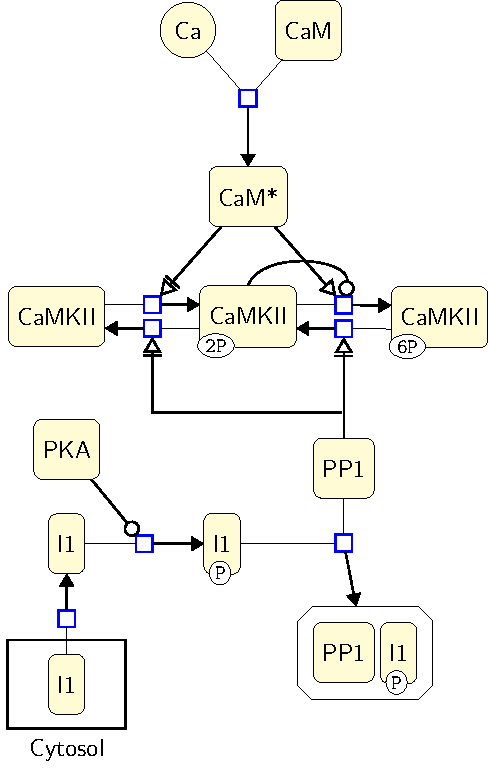
\includegraphics[width=\figW cm]{./model_sbgn_pd.pdf} 
    };
    \node[above=of model.north west,inner sep=1pt] (A) {\bf A};

    % B
    \node[inner sep=1pt] (B) at ([xshift=\colW cm]A) {\bf B};
    \node[below=of B.north west, anchor=north west,xshift=5mm] (reac) 
    {
        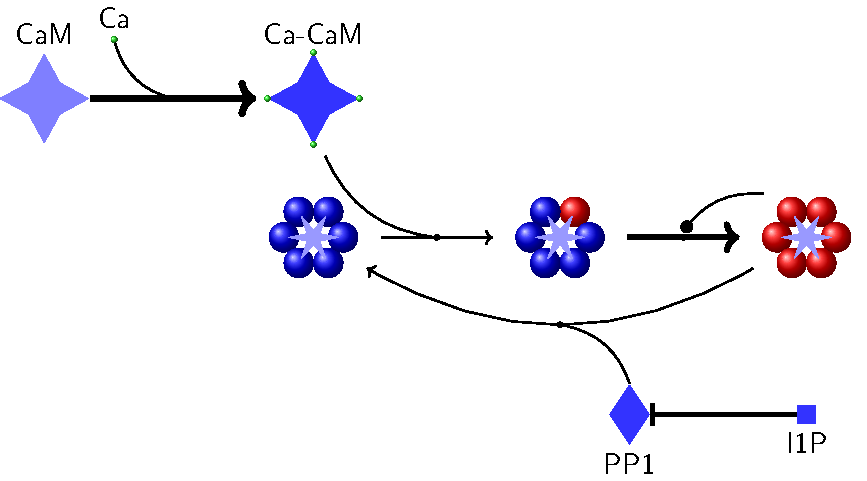
\includegraphics[width=\figW cm]{./camkii_pp1_switch_level1_detail.pdf} 
    };

    \node[below=of reac.south west, anchor=north west, yshift=0cm] (su) {
        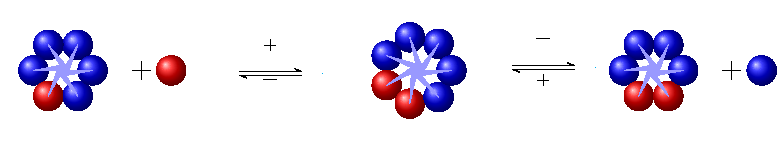
\includegraphics[width=\figW cm]{./camkii_subunit_exchage.pdf}
    };

    % Side figure.
    \begin{axis}[ name=C
        , at={(su.south west)}, anchor=north west
        , yshift=-10mm
        , xshift=11mm
        , xlabel=Time, x unit=\si{\second}
        , title={Ca\textsuperscript{2+} input}
        , y unit=\si{\nano M}
        , width=\colBW cm, height=1.5*\plotH cm
        , enlarge y limits
        , enlarge x limits={abs=1}
    ]
        \addplot [blue, thick] gnuplot [ raw gnuplot ] {
            mod(x,y)=x-floor(x/y)*y;
            b=80;
            f(t)=(mod(floor(t),4)>=2)?b:b*(1+rand(0));
            plot [t=0:20] f(t);
        };
    \end{axis} 
    \LABELAXIS{C}{C}

    \node[anchor=north west] (D) at ([xshift=\colW cm]B.north west) {\bf D};
    \begin{axis}[name=cam15
        , at=(D.south west), anchor=north west, xshift=15mm, yshift=-5mm
        , width=\colBW cm, height=\plotH cm
        , xtick={0,0.5,1.0,1.5,2.0}
        , enlarge y limits
        , ylabel={CaMKII\textsuperscript{*}}
        , title={N\textsubscript{CaMKII}=15}
        , xlabel=Time, x unit=day
        ]
        \addplot [color=blue] gnuplot [ raw gnuplot ] {
            plot "./camkii_15_200_days.dat" every 5::::10000
            using (column("time")/86400/30):(column("CaMKII*")/15)
        };
    \end{axis}

    \begin{axis}[ name=cam35, at=(cam15.south west), anchor=north west, yshift=\VGapBetweenAxis
            , xlabel=Time, x unit=month
            , width=\colCW cm, height=\plotH cm
            % , xmin = 0, xmax = 120
            , xtick={20,40,60,80,100,120}
            , enlarge y limits
            , ylabel={CaMKII\textsubscript{*}}
            , title={N\textsubscript{CaMKII}=35}
            % , title style={at={(0.15,1)}}
        ]
        \addplot [color=blue] gnuplot [ raw gnuplot ] {
            plot "./camkii_35_long.dat" every 100 
            using (column("time")/86400/30):(column("CaMKII*")/35)
        };
    \end{axis}
    \begin{semilogyaxis}[ name=E
        , at=(cam35.south west), anchor=north west
        , yshift = \VGapBetweenAxis
        , xlabel = N\textsubscript{CaMKII}
        , width = 0.75*\colCW cm
        , ylabel = Residence time, y unit=day
        , legend style={font=\scriptsize,fill=white,at={(0.6,0.0)},anchor=south west}
        , enlargelimits, grid
        ]
        \addplot[only marks, blue, thick, mark size=2pt,mark=o] table 
            [col sep=comma,x=CaMKII,y=CramerTime] {./switch_stability.csv};
        \addplot [domain=5:40, blue, very thick, smooth, solid, no markers] {exp((x-8)/4.2)};
        \legend{Simulation data,fit $\exp{\left(\frac{N_\text{CaMKII}-8}{4.2}\right)}$}
    \end{semilogyaxis}
    \LABELAXIS{E}{E}

    \node at ([xshift=17.8cm]A.west) {.};
\end{tikzpicture}
\end{document}
